In this chapter we discuss the performance of our models and compare to similar 
works. The chapter is split into two main sections: In the first section we 
discuss the performance of our machine learning models, compare to other similar 
experiments discuss ways to improve the machine learning aspects of this thesis.
In the second section we discuss the physical implications we believe the success 
of these machine learning models could have. We also discuss possible implications 
of our attribute importance rankings. 
\section{Machine Learning}
In this section we discuss the machine learning aspects of the results in this thesis.
We analyze the pure performance of our models and discuss whether we believe it 
is possible to improve said performance.
\subsection{Model Selection}
\label{discuss model selection}
Section \ref{CAMELS-GB results}-\ref{Mixed results} 
all agree that performance is increased when introducing static attributes. In 
addition to this, we see that the ordinary LSTM models that treat the static 
attributes as time series are the highest performing models. We find it likely that 
this is due  to the decrease in model complexity in an EA-LSTM compared to an LSTM. 
For example, Mixed$_\text{ea-lstm}$ has 205057 trainable parameters (weights and 
biases), Mixed$_\text{lstm}$ has 285953 and Mixed$_\text{none}$ has 266497. The 
EA-LSTM is a less complex model than an ordinary LSTM trained without 
static attributes. The EA-LSTM's ability to come close to the performance of an 
LSTM using $~72\%$ of the trainable parameters is notable, however. It could imply 
that in most cases even a less complex model benefits from the additional information 
contained in the attributes.
\subsection{Overfitting}
We find few clear signs of overfitting in our selected models when comparing 
cross validated performance to test performance. Table 
\ref{results summary table} indicates 
similar performance between the cross validated models and the refit models 
validated on the test set. There are some discrepancies in the CDF plot of 
the performance of the models trained on CAMELS 
shown in Figure \ref{test cdf} (second from top), leading to a median NSE of 
0.65 on the test set as opposed to $0.68$ in the cross validated case. This small 
deviation could perhaps be explained by the findings of \citet{lstm_second_paper},
 which found that an ensemble of LSTM models performs better than a singular LSTM 
 because of nontrivial differences in performance caused by randomness in the 
 training process. For computational reasons we have chosen not to use model 
 ensembles anywhere in this thesis.

Aside from dropout, we employ no regularization methods on our models. \citet{lstm_third_paper} 
argues that there is evidence that adding so called "physical constraints" to 
models used on CAMELS could be helpful. This is argued because the LSTM models 
underperform compared to SAC-SMA on some basins. Here the paper compares SAC-SMA 
to an LSTM trained on all basins, training and validation split time series-wise 
and not basin-wise. SAC-SMA is a conceptual model and is therefore not usually seen 
as a "physical" model, so we do not think this argument is enough to support said 
notion. The fact that all our best models significantly underperform on 
several basins could be an indication that we need to implement more regularization. 
This regularization might as well be based on physical principles, in our opinion. 
The benefit of physical constraints are many, some of which are:
\begin{itemize}
\item Interpretability: Physical constraints could improve the physical interpretability 
of the LSTM.
\item Improved generalization: The goal of most machine learning regularization is 
to improve regularization by increasing bias and decreasing variance (see Figure 
\ref{Bias Variance rainfall}). Increasing bias using physical laws would fit well 
into the narrative of \citet{BiasVarianceVIC} and \citet{VICbench}, although from 
the opposite angle. These papers argue that process-driven models are often too 
statistically constrained, due to them being driven almost entirely by interpretable 
physical processes. \citet{VICbench} showed that VIC performs at a higher level 
when tuning more parameters than usual, as these parameters are often set to based 
on physical a-priori knowledge. This is analogous to the bias-variance trade-off 
in machine learning. An LSTM is much less constrained and therefore performs better, 
agreeing with the results of the aforementioned papers. By making LSTM models 
slightly more constrained (as worded by \citet{BiasVarianceVIC}) could then make 
them generalize successfully to more basins while still being powerful enough to 
learn necessary relationships between input variables.
\end{itemize}
We propose a simple physical constraint:
\begin{equation}
\bm{\hat{y}} = \text{LSTM}(\bm{x}),
\end{equation}
where $\bm{\hat{y}}$ now consists of three outputs: $\bm{y}_\text{discharge}$, 
$\bm{y}_\text{frost}$ and $\bm{y}_\text{radiation}$. These represent runoff, 
frost/snow and radiated water respectively. Only $\bm{y}_\text{discharge}$ would 
be treated as the actual input when calculating the original cost function 
(\ref{NSE loss}). We then introduce a long term frost storage variable $\bm{W}_\text{frost}$.
For each time step this storage variable is updated by 
\begin{equation}
    \bm{W}_\text{frost}^{t+1} = \bm{W}_\text{frost}^t + \bm{y}_\text{frost},
\end{equation}
where $t$ is the current time step.
When calculating the loss function, we now add a new term to (\ref{NSE loss}):
\begin{equation}
    L = \text{NSE}^* + \gamma \left|(\bm{y_\text{discharge}} - \bm{x}_\text{precipitation} 
    - \bm{y}_\text{radiation} - (\bm{y}_\text{frost} - \bm{W}_\text{frost}))\right|
    \label{physical constraint}.
\end{equation}
Here $\gamma$ is a hyperparameter that needs to be separately tuned. Our reasoning 
behind (\ref{physical constraint}) is that this cost function penalizes models for 
making predictions where there is more runoff than available precipitation, 
snow and frost. Our hypothesis is that this penalty should lead to less complex 
models that are less likely to predict unphysical behaviors, leading to 
fewer NSE scores below zero. 

\begin{figure}
\centering


%\tikzset{every picture/.style={line width=0.75pt}} %set default line width to 0.75pt        

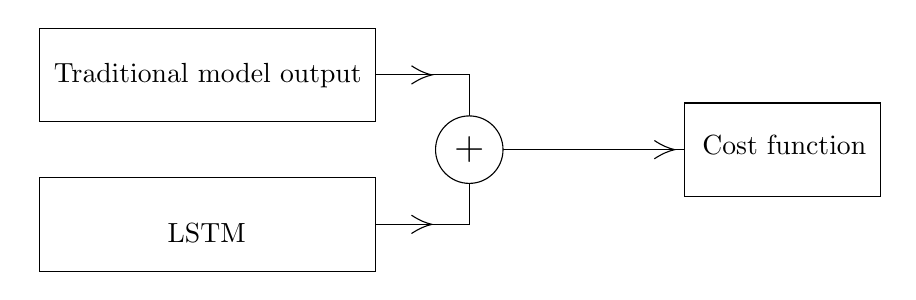
\begin{tikzpicture}[x=0.75pt,y=0.75pt,yscale=-0.9,xscale=0.9]
%uncomment if require: \path (0,300); %set diagram left start at 0, and has height of 300

%Shape: Right Angle [id:dp6736520719365272] 
\draw   (320,50) -- (370,50) -- (370,90) ;
%Shape: Right Angle [id:dp1824696211077277] 
\draw   (370,90) -- (370,130) -- (320,130) ;
%Straight Lines [id:da5169071611896188] 
\draw    (370,90) -- (485,90) ;
\draw [shift={(480,90)}, rotate = 180] [color={rgb, 255:red, 0; green, 0; blue, 0 }  ]   (10.93,-4.9) .. controls (6.95,-2.3) and (3.31,-0.67) .. (0,0) .. controls (3.31,0.67) and (6.95,2.3) .. (10.93,4.9)   ;
\draw [shift={(350,50)}, rotate = 180] [color={rgb, 255:red, 0; green, 0; blue, 0 }  ]   (10.93,-4.9) .. controls (6.95,-2.3) and (3.31,-0.67) .. (0,0) .. controls (3.31,0.67) and (6.95,2.3) .. (10.93,4.9)   ;
\draw [shift={(350,130)}, rotate = 180] [color={rgb, 255:red, 0; green, 0; blue, 0 }  ]   (10.93,-4.9) .. controls (6.95,-2.3) and (3.31,-0.67) .. (0,0) .. controls (3.31,0.67) and (6.95,2.3) .. (10.93,4.9)   ;
%\draw   (336,44.92) .. controls (340.03,47.37) and (344.07,48.84) .. (348.1,49.33) .. controls (344.07,49.82) and (340.03,51.3) .. (336,53.75) ;
%\draw   (338.5,130.08) .. controls (342.53,132.54) and (346.57,134.01) .. (350.6,134.5) .. controls (346.57,134.99) and (342.53,136.46) .. (338.5,138.92) ;

% Text Node
\draw    (140,25) -- (320,25) -- (320,75) -- (140,75) -- cycle  ;
\draw (230,50.2) node   [align=left] {\begin{minipage}[lt]{122.67200000000003pt}\setlength\topsep{0pt}
\begin{center}
Traditional model output
\end{center}

\end{minipage}};
% Text Node
\draw    (140,105) -- (320,105) -- (320,155) -- (140,155) -- cycle  ;
\draw (229.4,134.6) node   [align=left] {\begin{minipage}[lt]{122.67200000000003pt}\setlength\topsep{0pt}
\begin{center}
LSTM
\end{center}

\end{minipage}};
% Text Node
\draw  [fill={rgb, 255:red, 255; green, 255; blue, 255 }  ,fill opacity=1 ]  (370, 90) circle [x radius= 18.06, y radius= 18.06]   ;
\draw (370,90) node   [align=left] {\begin{minipage}[lt]{16.864pt}\setlength\topsep{0pt}
\begin{center}
{\Large +}
\end{center}

\end{minipage}};
% Text Node
\draw    (485,65) -- (590,65) -- (590,115) -- (485,115) -- cycle  ;
\draw (538.6,87.4) node   [align=left] {\begin{minipage}[lt]{68pt}\setlength\topsep{0pt}
\begin{center}
Cost function
\end{center}

\end{minipage}};


\end{tikzpicture}

.tex}
    \caption[Potential simple hybrid model.]{Sketch of how a simple hybrid model could be implemented. The traditional model and the LSTM model are completely separate, making it unnecessary to calculate gradients for the traditional model. The idea here would be for the LSTM model to learn the phenomena lacking in traditional models.}
\label{figure simple hybrid}
\end{figure}
Sticking to the topic of increased generalizability and interpretability, we 
believe it to be of interest to implement a hybrid model. 
By "hybrid model" we refer to a machine learning model implemented along side a 
traditional model. The machine learning model either replaces parts of or supplements 
the predictions of a traditional model. A very simple implementation of this is shown 
in Figure \ref{figure simple hybrid}. This model would take the same inputs as 
the models trained in this thesis, but the cost function would be calculated on 
the sum of the output of a traditional model and the machine learning model. 
What this essentially means is that the machine learning model learns to correct 
the errors of a given traditional model instead of doing all the prediction by 
itself.

 What we can view as overfitting is the case of transfer learning. Figure 
 \ref{training progress transfer} indicates that Transfer$_\text{GB, none}$ 
 and Transfer$_\text{US, none}$ start overfitting on their respective training 
 datasets. This overfitting isn't apparent when validating on basins from the 
 same dataset as they are trained on, but very quickly manifests when validating 
 on the other dataset. We view it as likely that if CAMELS-GB and CAMELS were to 
 have a perfectly overlapping supply of input data, it would show that this is 
 still the case for this case as well. This could indicate that training LSTM models 
 for transfer learning between different datasets either needs improved pre-processing, 
 or the introduction of further regularisation. It could also be that more data is needed.

 This and earlier research done by \citet{lstm_first_paper,lstm_second_paper,lstm_third_paper} 
 are all limited to simple LSTM models. LSTM models are, due to their recurrent nature, 
notoriously slow. Graphics cards and similar highly parallel computational devices 
are much more efficient for calculating less recurrent models. A relatively 
simple way to surpass this could be to implement a one dimensional 
Convolutional Neural Network (CNN) layer as the first layer of our model. This 
layer could then be used to reduce the time resolution of the data, still retaining 
information. The usage of CNNs for time series prediction is becoming increasingly
wide spread \citationneeded. 

\subsection{Hyperparameter Tuning}
We do not spend significant time in this thesis tuning hyperparameters. Instead, 
we chose to use the hyperparameters derived by \citet{lstm_second_paper}. The one 
exception to this is in the case shown in Section \ref{CAMELS-GB results}. We found 
that using dropout in this case at best makes no difference and at worst slightly 
decreases performance. In some cases we also tested whether increasing the 
sequence length from 270 days to 365 days increases performance, but our results 
indicate that this leads to no performance difference. The lower sequence length, 
the lower memory requirement per batch size, so we decided to keep using 270 days. 

We acknowledge that it may be possible to further increase the performance on 
CAMELS-GB by doing a thorough hyperparameter tuning experiment, this is 
something that definitely should be done in the future. 
\section{Physical Aspects}
In this section we discuss the physical implications of our results and what could 
possibly be used in future process-driven models and potential hybrid process-driven 
and machine learning models.
\subsection{Static Attribute Analysis}
\label{discuss static attributes}
Table \ref{overfit table} shows among others \textbf{\texttt{Q95}} as the most 
important attribute for the overfit "proof of concept" model. This attribute is the 
95th percentile runoff value for the full runoff time series for a given basin, 
information directly derived from the expected outcome. 
Because of this, we believe it is 
safe to assume two things: 1: An LSTM model can learn which static attributes are 
the most important in CAMELS-GB, at least in the most obvious case. 2: The permutation test 
succeeds at deciding the most important static attribute in this case. These 
assumptions are therefore used to strengthen our confidence in the results from 
our other, non-overfit models. 

As the results presented in Section \ref{CAMELS-GB results} and \ref{CAMELS results} 
indicate that the many of the important attributes are derived directly from the 
input time series, it is likely that we cannot extract much new information from 
these as this information should be available in the time series already used by 
most models. The reason for this is being the case is likely connected to the 
nature of the LSTM training process and the sequence length. Looking into ways 
to further improve the long-term memory of an LSTM should be further explored 
in the future.

We believe other ways to rank attributes should also attempted 
in the future, however. \citet{lstm_second_paper} used a robustness test which 
involves gradually adding Gaussian noise to a feature and checking how much it 
affects model performance (DOUBLE CHECK THIS!!!). \citet{OrigCAMELSRanking} 
uses a different method involving blah blah. These two methods should also be 
attempted on CAMELS-GB in addition to the permutation test employed in this 
thesis.



\subsection{Feasibility of transfer learning}
The results in Section \ref{Transfer learning section} show that the models trained 
for transfer learning do not benefit from adding static attributes. We also see 
that the case of US$\rightarrow$GB significantly improves the opposite. This makes 
sense as Great Britain has much smaller climatic variance than the United States 
\citationneeded. We believe these two phenomena could be related. It is likely 
that the relatively lower performance from using static attributes comes from the 
fact that the datasets have different climatic conditions. There could also be 
room for improvement in how we preprocess both the attributes and the time series. 
As seen in Table \ref{transfer table} we assume that the temperature time series 
of CAMELS behave like symmetrical periodic functions, therefore leading to 
\begin{equation}
T_\text{average} \approx  \frac{T_\text{min}+T_\text{max}}{2}. \label{dumb assumption}
\end{equation}
Ideally, we need to have temperature as a time series for a given model to be able 
to properly model snow and frozen soil accumulation, which is very important for 
hydrologic models \citationneeded. The fact that models trained on both datasets 
still perform comparably to models trained on only one dataset seems to suggest 
that (\ref{dumb assumption}) isn't entirely destructive, however.
In the later stages of this thesis it was discovered that the average temperature 
is actually present in CAMELS. The older \citationneeded forcing data contains 
this information stored as duplicates in the maximum and minimum temperature time 
series. Due to time constraints, we are unable to train models utilizing this. 
This is likely a good start for those looking to improve transfer learning performance. 
The best outcome is likely to come from finding maximum and minimum temperatures 
for CAMELS-GB, however.

It seems to us that there are several angles to further tackle the issue of transfer 
learning. The first we stated above: Find maximum and minimum time series for 
CAMELS-GB. The second is to improve the preprocessing of static attributes to 
the point where one would hopefully see better performance with attributes than 
without. A third option is to try introducing additional datasets. If one were to 
train on two datasets and validate on a third it could perhaps lead to better 
generalization. 
\subsection{Comparison to traditional models}
We are able to reproduce the results of \citet{lstm_second_paper,lstm_third_paper}, our models 
trained on CAMELS perform significantly better than traditional models. In this 
thesis we compare to two process-driven models: VIC and NWM, and one conceptual 
model: SAC-SMA. 

What we additionally show in this thesis is that models trained on both CAMELS and CAMELS-GB 
also perform better on CAMELS than the addressed traditional models. This could 
be because the models are complex enough to recognize which dataset a given 
basin is from based on underlying signatures in either the time series or the 
static attributes. Perhaps this differentiation could stem from differences in 
data collection practice. 

One of many reasons why LSTM models perform better than traditional models on CAMELS in general
(CHECK IF OTHERS ALSO CLAIM THIS) \citationneeded could be that the LSTM 
models are better at modelling basins with special conditions leading to 
a rainfall-runoff ratio different from 1. When the rainfall-runoff ratio is lower 
than one it usually implies that the rainfall is either stored as snow or frozen 
soil, or that it is vaporized through photosynthesis in local vegetation \citationneeded. 
These processes are difficult to model compared to runoff directly caused by 
rainfall \citationneeded.
Our results may indicate that this could be the case.
Figure \ref{runoff ratio} shows that only the traditional models have 
a statistically significant linear relationship between performance and 
rainfall-runoff ratio. The relationships are generally weak, with a Pearson 
correlation $\in \left[ 0.24, 0.33 \right]$, but they are more apparent than 
for the LSTM models, where there exists no such linear relationship. The impact 
of this discovery is quite uncertain, however, as there is significant 
Spearman correlation (nonlinear correlation) for all the models, ranging 
$\in \left[ 0.31, 0.53 \right]$.
